\pagebreak
\section{Diagrammi di Sequenza}
Si usano per descrivere lo scambio di messaggi e dati tra oggetti, indicando
anche la sequenza temporale. Si può usare sia in \emph{fase di analisi} per formalizzare
la \emph{sequenza principale degli eventi} nei casi d'uso, oppure in \emph{fase di progettazione}
per mostrare i messaggi scambiati dalle componenti (e anche attori) nell'architettura.

Gli oggetti e attori sono rappresentati da un rettangolo che indica il ruolo
e/o il tipo (nel caso dell'oggetto). Dal rettangolo parte una linea verticale chiamata \emph{linea di vita}
dell'oggetto: è tratteggiata quando l'entità è inattiva, invece è continua e doppia quando è attiva (nel caso di un attore la sua linea di vita è sempre attiva).

\begin{figure}[H]
    \centering
    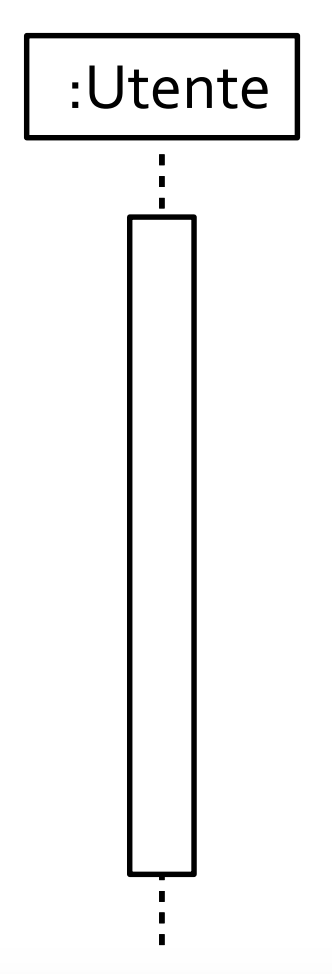
\includegraphics[scale=0.4]{img/sequenza.png}
\end{figure}

\paragraph{\textcolor{cyan}{Messaggi}} I messaggi rappresentano l'invocazione
di \emph{operazioni} o \emph{segnali}, possono essere:
\begin{itemize}
    \item Sincroni (\verb|1|)
    \item Di ritorno (\verb|1.1|)
    \item Asincroni (\verb|2|)
    \item Asincroni con esplicito uso di tempo (\verb|3|)
\end{itemize}

\begin{figure}[H]
    \centering
    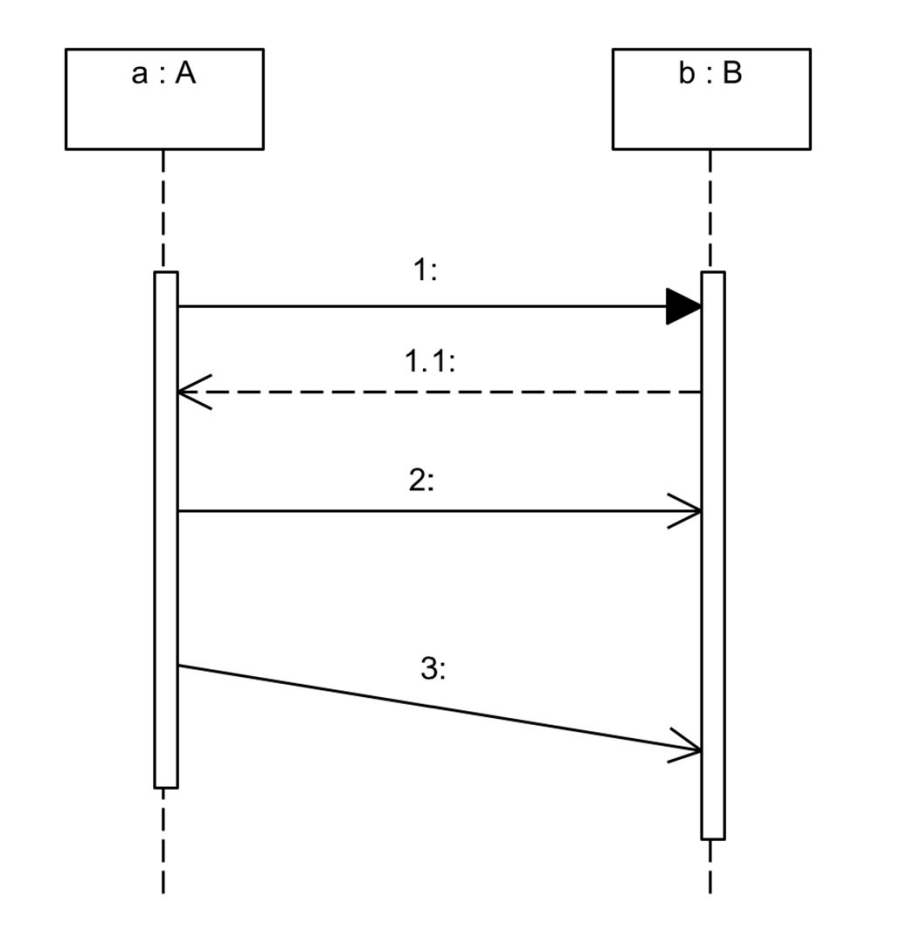
\includegraphics[scale=0.5]{img/messaggi_sequenza.png}
\end{figure}

Inoltre i messaggi presentano la seguente sintassi:

\begin{center}
    \verb|id: attributo = | \\
    \verb|nome_messaggio(arg1, arg2, ..., argN): valore_ritorno|
\end{center}

Le entità possono essere aggiunte e rimosse anche dinamicamente all'interazione.
Per la creazione si indica sulla freccia del messaggio la keyword \verb|<<create>>|.
Per la cancellazione, invece, si pone una $\times$ alla fine della sua linea di vita.


Nella linea di vita è possibile indicare anche vincoli di tempo o durata
per indicare un limite inferiore e/o superiore alla durata di un intervallo.

\paragraph{\textcolor{cyan}{Frame Condizionale}} È possibile dividere
il \emph{frame} del diagramma in più \emph{sottoframe}, ognuno dei quali
può avere una guardia (se non ne ha si assume che sia uguale a \verb|[true]|). In base
alla guardia che è vera (se ce n'è più di una la scelta è non deterministica) si
eseguono le azioni corrispondenti a quel sottoframe.

\paragraph{\textcolor{cyan}{Frame Iterativo}} Un frame può essere ripetuto più volte, si utilizza
la sintassi \verb|loop(min, max)|.

\begin{figure}[H]
    \centering
    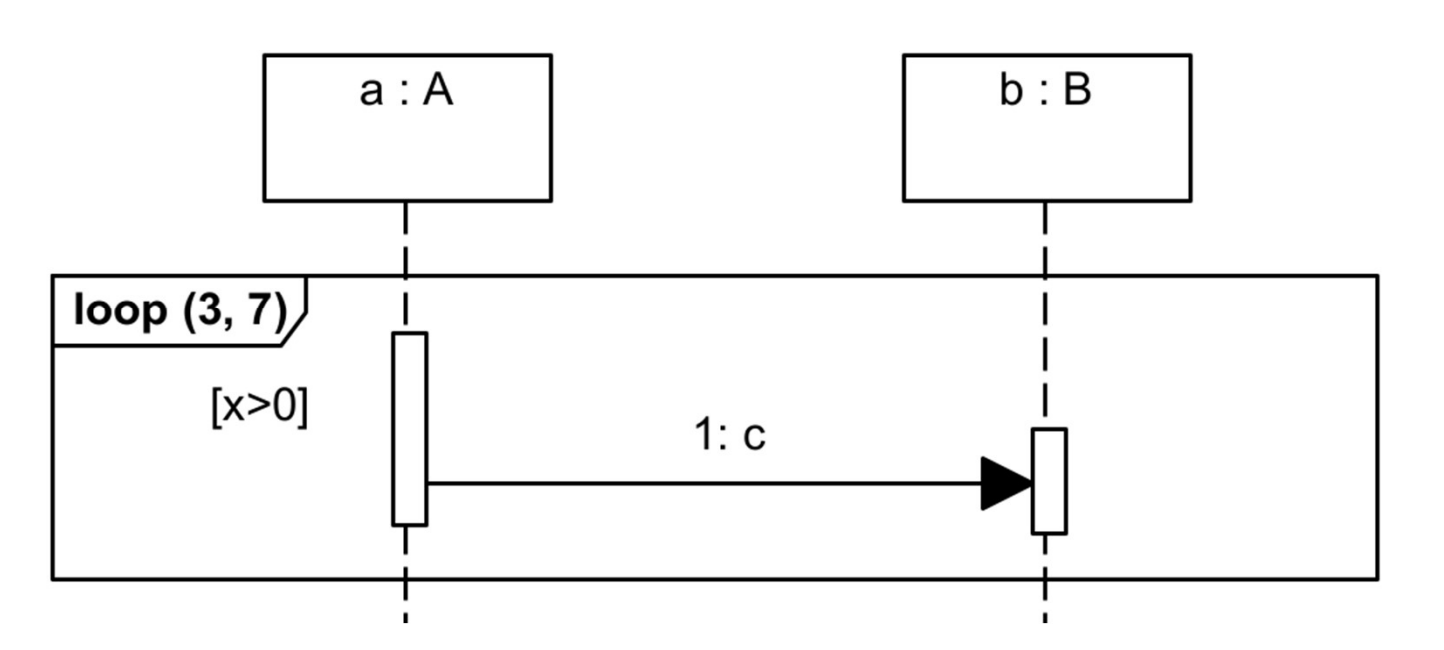
\includegraphics[scale=0.4]{img/frame_iterativo.png}
\end{figure}

\paragraph{Esempi.}

\begin{itemize}
    \item \verb|loop(0, *)[guardia]|: modella il \verb|while(guardia){...}|.
    \item \verb|loop(1, *)[guardia]|: modella il \verb|do{...}while(guardia)|.
    \item \verb|loop(n, n)| o \verb|loop(n)|: modellano un ciclo \verb|for| che và da $0$ a $n$ escluso.
\end{itemize}

\paragraph{\textcolor{cyan}{Frame Parallelo}} Le interazioni nei \emph{sottoframe} sono eseguiti
in parallelo (\emph{interleaving}).

\paragraph{\textcolor{cyan}{Ref}} È possibile includere in un frame un'interazione già definita tramite
l'indicatore \verb|ref| e scrivendo il nome del diagramma di sequenza da includere.

\paragraph{\textcolor{cyan}{Gates}} Un \emph{gate} è un punto sul bordo del diagramma a cui è
collegato un messaggio, o in ingresso o in uscita. Ogni gate ha un nome, e si utilizzano principalmente
quando si includono altri diagrammi.
